\documentclass{article}

\usepackage[final]{neurips_2019}

\usepackage[utf8]{inputenc}
\usepackage[T1]{fontenc}
\usepackage{hyperref}
\usepackage{url}
\usepackage{booktabs}
\usepackage{amsfonts}
\usepackage{amsmath}
\usepackage{nicefrac}
\usepackage{microtype}
\usepackage{graphicx}
\usepackage{xcolor}
\usepackage{lipsum}
\usepackage{float}
\usepackage{subfigure}

\newcommand{\note}[1]{\textcolor{blue}{{#1}}}

\title{
  Handwritten digit recognition using CNN\\
  \vspace{1em}
}

\author{
  Lu Baizhen (224040268) \\
  School of Data Science \\
  Chinese University of Hong Kong, Shenzhen \\
  \texttt{baizhenlu@link.cuhk.edu.cn} \\
  % Examples of more authors
  % \And
  % Name \\
  % School of Data Science \\
  % Chinese University of Hong Kong, Shenzhen \\
  % \texttt{name@cuhk.edu.cn} \\
  % \And
  % Name \\
  % School of Data Science \\
  % Chinese University of Hong Kong, Shenzhen \\
  % \texttt{name@cuhk.edu.cn} 
}

\begin{document}

\maketitle

\begin{abstract}
  This article investigates the current status of CNNs and some typical CNNs, 
  and implements handwritten digit recognition using a classic CNN: LeNet
\end{abstract}


% {\color{red} This template does not contain the full instruction set for this assignment; please refer back to the milestone instructions PDF.}

\section{Introduction}
The invention of Convolutional Neural Networks (CNNs) revolutionized the field of computer vision by enabling highly accurate, automated image recognition and classification. 
Comparing to traditional image processing methods, CNNs have higher accuracy and adaptability and have become the mainstream method in the field of computer vision.
In this report, the task is to implement a CNN for handwritten digit recognition using the famous CNN architecture LeNet.

\section{Related Work}
LeNet\cite{1998Gradient}, also called LeNet-5,which was invented in 1998,was the first CNN architecture to apply backpropagation to practical applications.
LeNet is composed of 2 convolutional layers, 2 mean pooling layers and 2 fully connected layers.
LeNet was first applied to handwritten character recognition at first and achieved good learning and recognition capabilities in postal code recognition, and is considered one of the origins of modern convolutional neural networks.
\begin{figure}[H]
  \centering
  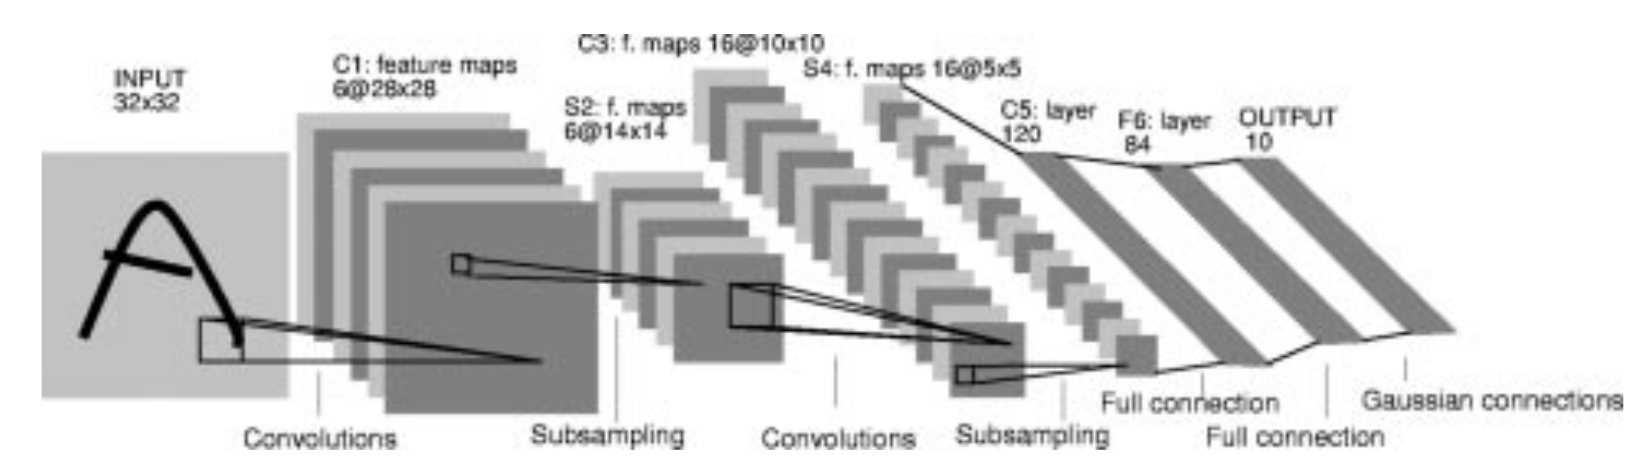
\includegraphics[width=0.8\linewidth]{./lenet.png}
  \caption{The architecture of LeNet}
\end{figure}
Due to the impact of computer performance, although LeNet has achieved good results in image classification, CNNs didn't attract much attention. 
In 2012, the AlexNet\cite{2012ImageNet} network proposed by Alex et al. won the ImageNet competition with a score far exceeding second place, and CNN and even deep learning have regained widespread attention.
AlexNet was also one of the first neural networks to use GPU for computation acceleration.
AlexNet is composed of 5 convolutional layers, 3 max pooling layers and 3 fully connected layers.
These years, one of the most famous computer vision systems for object detection is YOLO(You Only Look Once). 
\begin{figure}[H]
  \centering
  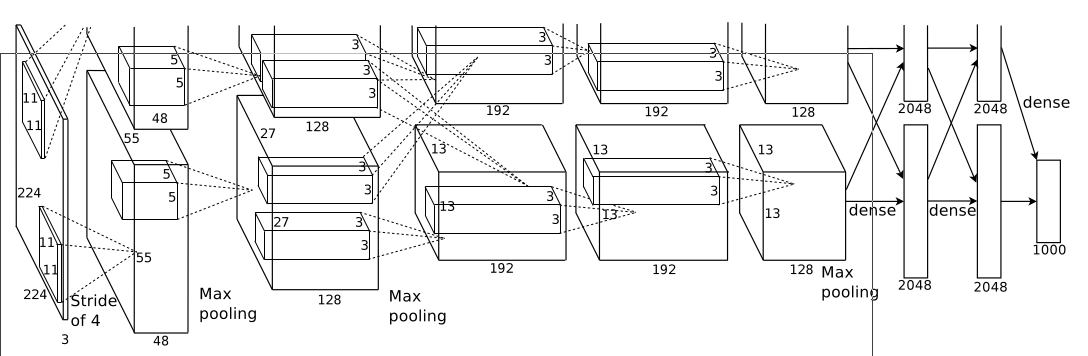
\includegraphics[width=0.8\linewidth]{./alexnet.png}
  \caption{The architecture of AlexNet}
\end{figure}
YOLO(You Only Look Once)\cite{redmon2016you} is a real-time object detection model that revolutionized the way objects are detected in images.
Unlike traditional methods, which treat object detection as a two-step process (region proposal followed by classification), YOLO frames it as a single regression problem.
It divides an image into a grid and simultaneously predicts bounding boxes and class probabilities for each grid cell, enabling fast, end-to-end object detection.
YOLO is known for its high speed and accuracy, making it suitable for real-time applications like autonomous driving, surveillance, and robotics.
The model has undergone several improvements through versions, including YOLOv2, YOLOv3, and YOLOv4, each offering better performance and efficiency.
\begin{figure}[H]
  \centering
  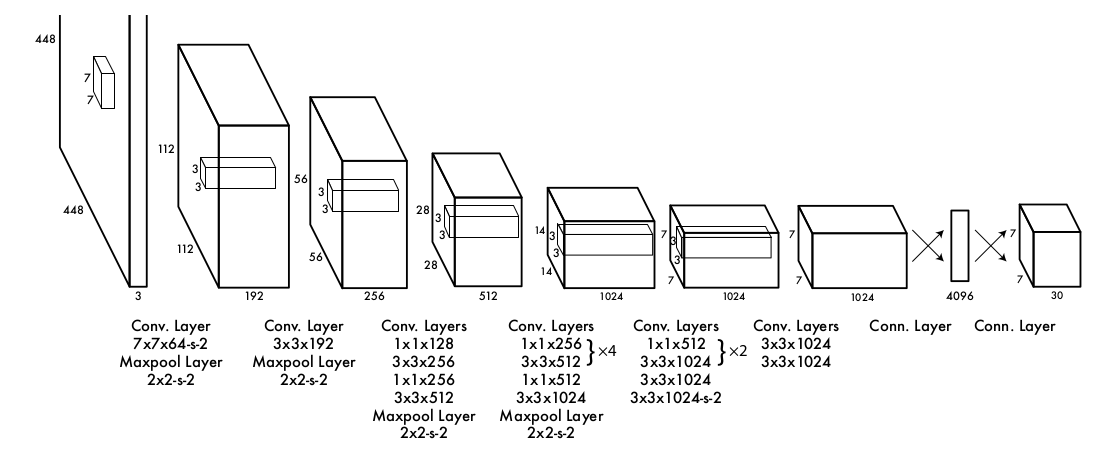
\includegraphics[width=0.8\linewidth]{./yolo.png}
  \caption{The architecture of YOLO}
\end{figure}

\section{Approach}
Use PyTorch
The components of LeNet used for recognizing grayscale images are as follows:
\begin{table}[h]
  \centering
  \begin{tabular}{c|c}
    Components & Property \\ \hline
    Conv1 & {input channels=1, output channels=6, kernel size=5, stride=1, padding=2} \\ 
    Sigmoid & - \\
    Pool1 & {kernel size=2, stride=2} \\
    Conv2 & {input channels=6, output channels=16, kernel size=5, padding=0} \\
    Pool2 & {kernel size=2, stride=2} \\
    Flatten & - \\
    {Linear1} & {input features = 400, output features = 120} \\
    {Linear2} & {input features = 120, output features = 84} \\
    {Linear3} & {input features = 84, output features = 10} 
  \end{tabular}  
\end{table}

\section{Experiments}
To train and validate the model, use the MNIST database of handwritten digits. Use cross entropy loss and Adam optimizer to train the model
\subsection{Data}
The MNIST database of handwritten digits contains 60000 examples for training and 10000 examples for testing.
The dataset contains 10 types of handwritten digit images ranging from 0 to 9, each of which has undergone size normalization and is a 28x28 grayscale image.
The dataset is randomly divided into a train set and a validation set in a 4:1 ratio.
\subsection{Evaluation method}
For binary classification, cross entropy loss is 
$$L = - [ y \cdot \log(p) + (1 - y) \cdot \log(1 - p) ]$$
For multi-class, it sums over all classes:
$$L = - \sum_{i} y_i \cdot \log(p_i)$$

\subsection{Experimental details}
For the data loader, the batch size is 64. The learning rate of Adam optimizer is 0.001. The epoch of training is 20.
The training process is accelerated using an Nvidia GTX1650 graphics card through CUDA.

\subsection{Results}
The training result is shown as below:
\begin{figure}[htbp]	
  \centering
	\subfigure[Loss] %第一张子图
	{
		\begin{minipage}{6cm}
			\centering          %子图居中
			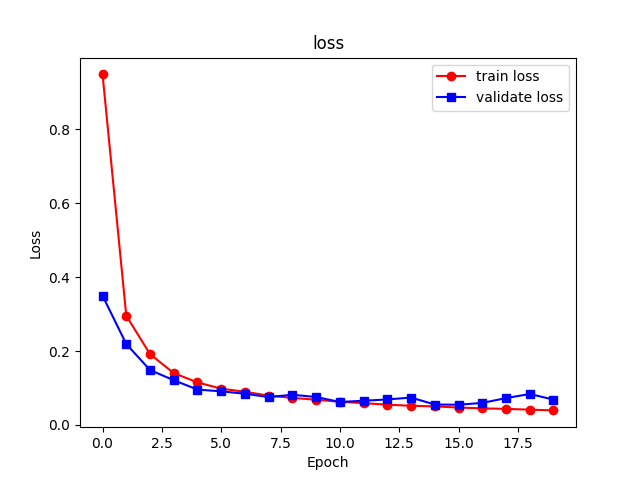
\includegraphics[scale=0.4]{loss.png}   %以pic.jpg的0.4倍大小输出
		\end{minipage}
	}
	\subfigure[Accuracy] %第二张子图
	{
		\begin{minipage}{7cm}
			\centering      %子图居中
			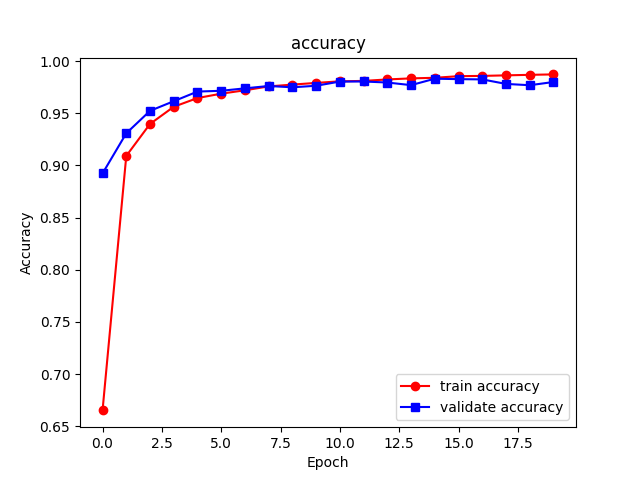
\includegraphics[scale=0.4]{acc.png}   %以pic.jpg的0.4倍大小输出
		\end{minipage}
	}
	\caption{Training result} %  %大图名称
\end{figure}

After the 20th epoch,
Train Loss=0.0397, Train Accuracy=0.9879, Validate Loss=0.0552, Validate Accuracy=0.9836.
Training completed in 1m13s.

\section{Analysis}
The loss and accuracy converged quickly during the first 3 epochs in the training.
After the training, the accuracy of the model is at a very high level.

\section{Conclusion}

LeNet is a relatively simple but efficient and accurate model.
It has demostrated good performance in handwritten digit recognition tasks. 

\newpage
\bibliographystyle{unsrt}
\bibliography{references}

\end{document}

